% !TeX root = dissertation.tex
\chapter{Background}
\label{chapter:background}

Bugnion, Nieh and Tsafrir~\cite{bugnion-nieh-tsafrir} define virtualization as
\textit{``the application of the layering principle with enforced modularity
such that the exposed resource is identical to the underlying resource''}.
To put it in simpler words, virtualization is about controlling the interface
to a hardware resource (\emph{interposition}) in order to multiplex it among
multiple users in a safe manner (\emph{isolation}), without any of them being
the wiser (\emph{compatibility}). Virtualization is a huge area with a long
and storied history, as alluded to in the introduction;
see \textit{Bugnion, Nieh and Tsafrir}'s \textit{Hardware and software support for virtualization}~\cite{bugnion-nieh-tsafrir} for comprehensive treatment.

\section{Virtualization Properties}
\label{s:properties}

Given our focus accelerator virtualization, let us consider the following key
properties: \emph{interposition}, \emph{compatibility}, and \emph{isolation}.

\textbf{Interposition.}
Virtualization decouples a logical resource from a physical one
through an indirection layer, intercepting guest interactions with
a virtual resource and providing the requested functionality using
a combination of software and the underlying physical resource.
Thus, virtualization works by \emph{interposing}
an interface, and changing or adding to its behavior.
Interposition is fundamental to virtualization and provides well-known benefits~\cite{waldspurger12cacm}.
The choice of interface and the mechanism for interposing it
profoundly impacts the resulting system's practicality.
\emph{Inefficient} interposition of an interface (e.g. trapping frequent MMIO access) undermines
performance~\cite{suzuki2014gpuvm,yu2017fullvirt}; \emph{incomplete} interposition
compromises the hypervisor's ability to enforce isolation.

\textbf{Compatibility} as applied to virtualization captures multiple related
dimensions, from robustness to evolution of interposed interfaces and adjacent
stack layers, to applicability across multiple platforms or related devices.
For example, full virtualization of a accelerators's hardware interface
 has \emph{poor} compatibility in that it works only with
that device. However, it has \emph{good} compatibility with guest software,
which will work without modification, assuming the operating system has
appropriate drivers for the device.
Current accelerator virtualization techniques
reflect a compromise between these two forms of compatibility.


\textbf{Isolation.}
Cross-VM isolation is a critical requirement for multi-tenancy:
when a resource is multiplexed among mutually distrustful tenants, tenants
must not be able to see/alter each other's data (\emph{data isolation}),
or adversely affect each other's performance (\emph{performance isolation}).
A poor choice of interposition mechanism and/or interface limits the system's
ability to provide these guarantees:
e.g., API remoting~\cite{bitfusion, rCUDA, mps} has poor isolation in the
common case, as the hypervisor is bypassed. Using separate servers for each
protection provides isolation.

\section{Domain Specific Accelerators}
Domain Specific Accelerators (DSAs) are programmable compute units that are
specialized to a particular class of computation in order to improve
performance, to optimize energy usage for that class of computation, or
frequently both.
The slowing down of Moore's law coupled with the rise of Dark Silicon~\cite{
Esmaeilzadeh2011-qv} has made Domain Specific Accelerators extremely attractive
as they exhibit high computation/Watt efficiency in the computation domain
they are specialized to. For example, consider Google's Tensorflow Processing
Unit (TPU)~\cite{TPU-CACM}, a DSA for the Tensor-based computation popular in
Neural Networks.
The first generation of TPUs were empirically found to have 200$\times$ and
79$\times$ higher Performance/Watt respectively over the CPUs and Nvidia k80
GPUs that were prevalent in Google's data centers at the time~\cite{TPU-ISCA}.

\subsection{DSA Design}
Domain Specific Accelerators are mini-computers that are attached to and
controlled by a CPU. DSAs tend to have everything a normal 'computer' does (
computation units, control logic, memory, and a programming interface), except
access to I/O, for which they typically rely on the CPU.
Their computation units are typically specialized to a specific domain or type
of computation: e.g., GPUs are DSAs that are specially suited to graphics
rendering operations (tesselation, occlusion detection, culling, etc.).
GPUs have also found wider adoption in other domains (scientific computing,
Artificial Intelligence, etc.) due to their inclusion of Single Instruction
Multiple Thread (SIMT) style `shader' cores, which efficiently perform
the same simple computation in parallel on hundreds (or even thousands) of
threads. DSAs typically have their own memory: while some have small amounts
of memory that are just enough to process limited operations (e.g., Intel
QAT), most have a lot of internal memory, as memory bandwidth and size are key
parameters in tuning the architecture for the given domain. DSAs typically
expose an I/O device-like hardware interface, i.e., a command queue, a DMA
engine, and some number of memory-mapped control registers.

DSAs look like I/O devices to the host CPU, and many DSA designers take
advantage of this to build a software stack that is opaque to the host OS.
Exposing an I/O device-like hardware interface enables the vendor to raise the
level of abstraction of the end user's interface to a user-space software API,
enabling quick evolution of both the underlying software and hardware. The
user-space API is the only interface that needs to be stable (or at least
backwards compatible). The ISA of the compute units on the DSA are typically
not exposed to the programmer.

\subsection{DSA Software stacks are silos}
\begin{figure}[!h]
	\centering
	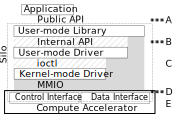
\includegraphics[width=.5\linewidth]{figures/silo.pdf}
	\caption{An accelerator silo. The public API and the interfaces with striped backgrounds are interposition candidates. All interfaces with backgrounds are proprietary and subject to change.}
	\label{fig:silo}
\end{figure}

Domain Specific Accelerator stacks are composed of layered components that
include a user-mode library to support an API framework and a driver to manage
the device. Vendors are incentivized to use proprietary interfaces and
protocols between layers to preserve forward compatibility, and to use
kernel-bypass communication techniques to eliminate OS overheads.

Scheduling and resource allocation on DSAs are typically not managed by the
CPU-based Operating System. Instead resource allocation is primarily under the
control of a combination of the proprietary CPU-based runtime (user-space and
kernel), and the controller on the DSA itself. DSAs typically contain an
entire software stack on the hardware module, which is hidden from the
programmer. This stack is used to implement a command-based programming
interface that enables the vendor's CPU-based control software for scheduling
and resource allocation.

End users work with the DSA almost entirely in higher level languages,
typically the language the DSL is embedded in (e.g., Python for Google's TPU,
C/C++ for Nvidia and AMD GPGPUs). The DSL/API is supported by a compiler
(which converts the user's program to the the ISA of the computation units on
the DSA), a user-space runtime and a kernel module (which work together to
implement the user-space API, and control the DSA).

\section{DSA Virtualization}

Despite mounting evidence of accelerator under-utilization~\cite{
underutilizingcloud, simultaneous_multikernel,improving_gpu,gpl,fiddle},
and abundant prior research into multiplexing Domain Specific Accelerators
(DSAs)~\cite{gpl,fiddle,zhang2018g, simultaneous_multikernel,improving_gpu,
yeh2017pagoda}, DSAs remain dedicated exclusively to a single guest in shared
computing environments. This section provides background on the well studied,
but mostly unresolved problem of GPGPU virtualization to explain this trend.

Existing GPU virtualization solutions~\cite{dowty2009gpu, VGML} support
graphics frameworks like Direct3D~\cite{directX}, OpenGL~\cite{openGLspec}.
In principle, there should be no fundamental difference between GPU
virtualization for graphics versus \emph{compute} workloads, as ``compute
shaders'' are implemented by the hardware as an additional stage in the
graphics pipeline~\cite{gpu_shader}.
In practice, they have significantly different goals:
for graphics, virtualization designs target an interactive frame rate (18-30
fps~\cite{frame_rate}); for GPGPU compute, virtualization designs must
preserve the raw speedup achieved by the hand-optimized GPGPU application,
which is a considerably harder target to hit. As a result, GPGPU virtualization
remains an open problem. While graphics devices have long enjoyed well-defined
OS abstractions and interfaces~\cite{winGDI}, research attention to OS
abstractions for GPGPUs~\cite{rossbach2011ptask, dandelion,
silberstein2013gpufs, timegraph, gdev, gpunet} has yielded little consensus.
Persistent vendor-specificity of programming frameworks further impedes both
interposition and compatibility.

\subsection{Inefficacy of Traditional GPGPU Virtualization Techniques}
An ideal GPGPU virtualization design would require no modification of
guest applications, libraries and OSes (compatibility), arbitrate fair and
isolated sharing of GPU resources between mutually distrustful VMs (sharing
and isolation) at the native performance of the hardware (performance), while
allowing virtualized software and physical hardware to evolve independently
(encapsulation).
We briefly describe each technique, and look at their strengths and
shortcomings in this section. Refer to Related Work (\S~\ref{sec:related}) for
details on individual prior work under each technique.

\subsubsection{Pass-through}
PCIe pass-through, the current \emph{de facto} standard technique for GPGPU
virtualization, provides a VM with full exclusive access to a physical GPU.
The GPU's hardware interface is directly exposed to the guest OS, and
therefore can't be multiplexed as the hypervisor does not interpose \emph{any}
interface. Virtualization hardware extensions (e.g., Intel VT-d~\cite{
abramson2006intel}) are device-agnostic, making PCIe pass-through easily
adaptable to any DSA. Pass-through provides native performance at the cost of
\emph{sharing, interposition, compatibility and isolation}.

\subsubsection{Device emulation}
Device Emulation~\cite{bellard2005qemu} provides a full-fidelity
software-backed virtual device which yields excellent compatibility,
interposition, and isolation. However, device emulation can't support hardware
acceleration making it untenable for virtualizing GPGPUs.

\subsubsection{Full virtualization}
The hypervisor interposes GPU's hardware interface to provides a virtual
environment in which unmodified GPGPU programs run on unmodified guest
software stacks.
For DSAs, this interface tends to be memory mapped I/O (MMIO), necessitating
trap-based interposition (e.g. using memory protection or de-privileging),
leading to devastating performance slowdowns (e.g., 100$\times$ slowdown with
GPUvm~\cite{suzuki2014gpuvm,yu2017fullvirt}). DSA hardware interfaces tend to
be proprietary and device-specific, so full virtualization based solutions
have poor compatibility, even across different devices of the same type (e.g.
AMD vs NVIDIA GPUs). Full virtualization solutions also typically rely on
reverse engineering of proprietary control interfaces, rendering them
extremely tedious to build, maintain and evolve.

\subsubsection{Mediated pass-through}
A hybridization of pass-through and full virtualization, Mediated
pass-through~\cite{gVirt,mdev-mvme,vpio} uses pass-through for data plane
operations, and provides a privileged control plane interface for sensitive
operations. Mediated pass-through can preserve some of the raw speedup of
acceleration and allows guests to use native drivers and libraries.
However, limited interposition limits a hypervisor's ability to effectively
manage resource sharing. More importantly, hardware support is required. To
our knowledge, Intel integrated GPUs are the only accelerators with such
support.

\subsubsection{Para-virtualization}
Rather than interposing an existing interface in the stack,
para-virtualization~\cite{suzuki2014gpuvm,dowty2009gpu,vasila-gvm16,
vmm-independent-gfx-vee07,harel-efficient13atc,exitless-paravirtual-io,
vmm-bypass-atc06, self-virt-hpdc07,vmware-hosted-io-atc01,
direct-access-virt-io-atc08, paradice} \emph{creates} an efficiently
interposable interface in software and adjusts adjacent stack layers to use
it. The driver and runtime libraries in every supported OS must be
modified to work in concert with the virtualization layer.
Para-virtualization enables encapsulation of diverse hardware behind a single
interposable interface, but compromises compatibility. Guest software must be
modified, and the para-virtual device interface must be maintained as
interfaces evolve.
For example, VMware's SVGA II~\cite{dowty2009gpu} encapsulates multiple GPU
programming frameworks, but keeping up with the evolution of those frameworks
has proved untenable: SVGA remains multiple versions  behind current
frameworks~\cite{vmware_version,svga_guest}.

\subsubsection{API Remoting}
User-space API Remoting based virtualization designs interpose
application-level APIs (e.g. CUDA, OpenCL) by shimming a dynamic library and
remote them to the corresponding framework in the host~\cite{shi2012vcuda,
gupta2009gvim, gVirtuS}, on a dedicated appliance VM~\cite{vmCUDA}, or on a
remote server~\cite{rCUDA,rCUDAnew,GridCuda,kim2012snucl,VCL,Duato2009,Li2011}.
API Remoting is similar to RPC~\cite{nfs,sunrpc} or system call
interposition~\cite{paradice, nooks, rio, vrio}.
Limited interposition frequency, batching opportunities~\cite{rCUDA} and
high-speed networks~\cite{deplyrcuda, bitfusion} reduce overheads, making this
class of designs appealing to industry. Dell XaaS~\cite{xaas}, BitFusion
FlexDirect~\cite{bitfusion}, and Google Cloud TPUs~\cite{cloud-tpu} currently
use it to support GPUs, FPGAs, and TPUs.
However, API remoting compromises compatibility if multiple APIs or API
versions must be supported. Moreover the technique bypasses the hypervisor,
giving up the interposition required for hypervisor-enforced resource
management. Our experiments with commercial systems like BitFusion
FlexDirect~\cite{bitfusion} show vulnerability to massive unfairness
pathologies. Figure~\ref{fig:bitfusion_unfairness} shows the problem on an
NVIDIA GTX 1080: FlexDirect is unfair (up to 88.1\%) when running two
applications with different kernel run-lengths (126.3~ms/kernel vs 0.18~ms/
kernel in the worst case).

\begin{figure}[!t]
	\centering
	\includegraphics[width=.8\linewidth]{figures/bf_unfairness.pdf}
	\caption{Unfairness in slowdown between \lstinline|needle| and \lstinline|hotspot| applications in separate VMs running GPU kernels iteratively
    with BitFusion FlexDirect.
    When running alone, \lstinline|hotspot| has throughput of 126.3~ms/kernel.
    Fairness is calculated by $\left|s_1-s_2\right| \mathbin{/} (s_1+s_2),$
    where $s_i$ is the slowdown of application $i$ when running concurrently.
    \aak{remove AVA from this figure.}}
	\label{fig:bitfusion_unfairness}
\end{figure}

Deferring enforcement to a trusted surrogate in the host or remote machine is
a tenable alternative. However, the co-ordination required to integrate with
hypervisor-level resource management means that current solutions do not
support it, and the engineering effort required would be substantial.
Existing accelerator API remoting systems are by themselves massive
undertakings without any hypervisor integration: systems like Bitfusion
FlexDirect~\cite{bitfusion}, and rCUDA~\cite{rCUDA} reflect multi-year
system-building efforts.

\subsubsection{Hardware virtualization support}
Hardware support for virtualization (e.g., Single Root I/O Virtualization (
SR-IOV)) enables a single physical device to present itself as multiple
virtual devices. A hypervisor can manage and distribute these virtual devices
to guests, effectively deferring virtualization, scheduling, and resource
management to the hardware. NVIDIA and AMD both ship GPU cards targeted at the
VDI market that use SR-IOV to export multiple virtual GPUs from the hardware.

SR-IOV exhibits close to native performance~\cite{XenSRIOV}, but this is
achieved at the cost of interposition --- the hypervisor can't interpose
on any interactions with the hardware. SR-IOV also suffers from the multiple
administrator problem: the hardware controller and the hypervisor/OS may make
mutually inconsistent decisions leading to unpredictable behavior.
SR-IOV provides an interface and protocol for managing VFs, but the device
vendor must \emph{implement} any cross-VF sharing support \emph{in silicon}.
The technique can provide strong virtualization guarantees~\cite{dong2012high,
dong2008sr}, but hardware-level resource management is inflexible and slow to
evolve: current implementations are trivially vulnerable to fragmentation and
unfairness pathologies that cannot be changed.

\begin{figure}[!t]
	\centering
  \vspace{-0.5em}
	\includegraphics[width=.75\linewidth]{figures/qat_unfairness.pdf}
    \vspace{-.2cm}
	\caption{Throughput achieved by three instances of QATzip (running in VMs with SR-IOV pass-through) with different block sizes, running separately (\textbf{\texttt{Uncontended}}) and concurrently (\textbf{\texttt{Contended}}). Slowdown during concurrent execution is dependent on block size, i.e., the QAT HW scheduler cannot guarantee fairness.}
	\label{fig:qat-unfairness}
\end{figure}

Hardware designers tend to favor simple resource management policy
implementations, easily leading to pathologies. To illustrate the problem, we
measured compression throughput when three VMs contend on an Intel
QuickAssist~\cite{qat} (with SR-IOV). The three VMs configured the accelerator
to compress at different chunk sizes. Figure~\ref{fig:qat-unfairness} shows
the results of this experiment, with and without contention. Each VM was
assigned a PCIe Virtual Function (VF) exposed by the same Physical Function
(PF), causing the hardware to schedule requests round-robin. When there is no
contention, each application achieves a similar throughput. However, when the
3 applications were executed concurrently, the throughput achieved was a
function of offload chunk size used, \emph{yielding unfairness that cannot be
fixed without changing the hardware}.

Further, evidence is scant that broad SR-IOV support will emerge for
accelerators: only two current GPUs support it~\cite{amdfirepro,nvidiagrid},
none of the TPUs we evaluate support it; and SR-IOV \emph{interface} IP blocks
from FPGA vendors (used by~\cite{vu2014enabling,zazo2015pcie,vfpgamanager,
huang2009fpgavirt}) do not implement resource management.

\section{Summary}

Interposing opaque, frequently-changing interfaces communicating with memory
mapped command rings is \emph{impractical} because it requires inefficient
techniques and yields solutions that sacrifice compatibility.
Accelerator stacks are effectively \emph{silos} (Figure~\ref{fig:silo}), whose
intermediate layers \emph{cannot be practically separated} to virtualize the
device. Most current hardware accelerators feature some hardware support for
virtualization: primarily for process-level address-space separation, and in a
small handful of cases, SR-IOV. A central premise of this dissertation is that
hardware support for process-level isolation \emph{could} suffice to support
hypervisor-level virtualization as well, but the silo-ed structure of current
accelerator stacks prevents it.
While hardware support for virtualization is the desired end game, we do not
expect a better standard for such support to emerge soon: incentives for
investing in the significant engineering effort required for such a standard
are scarce. This dissertation focuses on virtualization schemes that can be
purely implemented in software so as to sidestep this challenge.